\begin{filecontents*}[overwrite]{o5s-references.bib}
@misc{o5s, author={{o5s contributors}}, title={{o5s}: Source, proofs, and recorded measurements at commit d615e77}, year={2026}, url={https://github.com/h5i-dev/o5s/tree/d615e77c60995137ddb47b0bd56544143d76a01c}, note={Pinned artifact; full revision d615e77c60995137ddb47b0bd56544143d76a01c}}
@misc{cfgit, author={Dina Kozlov and Dillon Mulroy and Zebulon Piasecki}, title={We want you to build the next Git platform on Cloudflare}, year={2026}, month=oct, howpublished={The Cloudflare Blog}, url={https://blog.cloudflare.com/next-git-platform-on-cloudflare/}, note={October 1, 2026}}
@misc{h5i, author={{h5i contributors}}, title={h5i: The agent-native web security workspace}, year={2026}, url={https://github.com/h5i-dev/h5i}, note={Includes the h5i-app framework (crates h5i-app 0.1.1 and companions); accessed October 12, 2026}}
@misc{charon, author={{AeneasVerif}}, title={Charon: Interface with the rustc internals}, year={2026}, url={https://github.com/AeneasVerif/charon}, note={Accessed October 12, 2026}}
@misc{gitobjects, author={{Git project}}, title={Git Internals: Git Objects}, year={2026}, url={https://git-scm.com/book/en/v2/Git-Internals-Git-Objects}, note={Undated Pro Git documentation; accessed October 12, 2026}}
@misc{gitrebase, author={{Git project}}, title={git-rebase: Reapply commits on top of another base tip}, year={2026}, url={https://git-scm.com/docs/git-rebase}, note={Undated online manual; accessed October 12, 2026}}
@misc{darcs, author={{Darcs project}}, title={Darcs Theory}, year={2026}, url={https://darcs.net/Theory}, note={Undated project documentation; accessed October 12, 2026}}
@misc{pijul, author={{Pijul project}}, title={Pijul Manual: Theory}, year={2026}, url={https://pijul.org/manual/theory.html}, note={Undated project documentation; accessed October 12, 2026}}
@misc{jj, author={{Jujutsu contributors}}, title={First-class conflicts}, year={2026}, url={https://docs.jj-vcs.dev/latest/conflicts/}, note={Undated project documentation; accessed October 12, 2026}}
@article{patches, author={Samuel Mimram and Cinzia Di Giusto}, title={A Categorical Theory of Patches}, journal={Electronic Notes in Theoretical Computer Science}, volume={298}, pages={283--307}, year={2013}, doi={10.1016/j.entcs.2013.09.018}, url={https://arxiv.org/abs/1311.3903}}
@article{aeneas, author={Son Ho and Jonathan Protzenko}, title={Aeneas: Rust Verification by Functional Translation}, journal={Proceedings of the ACM on Programming Languages}, volume={6}, number={ICFP}, articleno={116}, numpages={31}, pages={711--741}, year={2022}, doi={10.1145/3547647}, url={https://arxiv.org/abs/2206.07185}}
@inproceedings{lean, author={Leonardo de Moura and Sebastian Ullrich}, title={The Lean 4 Theorem Prover and Programming Language}, booktitle={Automated Deduction -- CADE 28}, series={LNCS}, volume={12699}, publisher={Springer}, pages={625--635}, year={2021}, doi={10.1007/978-3-030-79876-5_37}, url={https://lean-lang.org/papers/lean4.pdf}}
@misc{gitcve, author={Taylor Blau}, title={Git security vulnerabilities announced}, year={2025}, month=jul, howpublished={The GitHub Blog}, url={https://github.blog/open-source/git/git-security-vulnerabilities-announced-6/}, note={July 8, 2025; updated July 28, 2025}}
@misc{githubcve, author={Alexis Wales}, title={Securing the git push pipeline: Responding to a critical remote code execution vulnerability}, year={2026}, month=apr, howpublished={The GitHub Blog}, url={https://github.blog/security/securing-the-git-push-pipeline-responding-to-a-critical-remote-code-execution-vulnerability/}, note={April 28, 2026; updated April 29, 2026}}
@misc{gitlabcve, author={{GitLab}}, title={GitLab Critical Patch Release: 17.3.3, 17.2.7, 17.1.8, 17.0.8, 16.11.10}, year={2024}, month=sep, url={https://docs.gitlab.com/releases/patches/patch-release-gitlab-17-3-3-released/}, note={September 17, 2024}}
@misc{hf, author={{OpenAI}}, title={The Hugging Face incident and the road ahead}, year={2026}, month=aug, url={https://openai.com/index/hugging-face-incident-and-the-road-ahead/}, note={August 26, 2026}}
@article{sec, author={Victor B. F. Gomes and Martin Kleppmann and Dominic P. Mulligan and Alastair R. Beresford}, title={Verifying Strong Eventual Consistency in Distributed Systems}, journal={Proceedings of the ACM on Programming Languages}, volume={1}, number={OOPSLA}, articleno={109}, numpages={28}, year={2017}, doi={10.1145/3133933}, url={https://arxiv.org/abs/1707.01747}}
@inproceedings{homotopical, author={Carlo Angiuli and Edward Morehouse and Daniel R. Licata and Robert Harper}, title={Homotopical Patch Theory}, booktitle={Proceedings of the 19th ACM SIGPLAN International Conference on Functional Programming}, series={ICFP '14}, pages={243--256}, year={2014}, publisher={ACM}, doi={10.1145/2628136.2628158}, url={https://www.cs.cmu.edu/~rwh/papers/htpt/paper.pdf}}
\end{filecontents*}
\documentclass[sigconf,nonacm,pbalance=true]{acmart}
\usepackage{amsmath}
\usepackage{needspace}
\usepackage{booktabs}
\usepackage{enumitem}
\setlist[itemize]{leftmargin=1.2em,labelsep=0.4em,itemsep=1pt,parsep=0pt,topsep=2pt}
\usepackage{tikz}
\usetikzlibrary{arrows.meta,positioning}
\settopmatter{printacmref=false,printfolios=true}
\setcopyright{none}
\newcommand{\sys}{\textnormal{o5s}}
\newcommand{\code}[1]{\texttt{\small #1}}
\setlength{\emergencystretch}{1.5em}
\setlength{\parskip}{0pt plus 3pt}
\AtBeginDocument{\clubpenalty=150 \widowpenalty=150 \displaywidowpenalty=150}
\renewcommand{\figurename}{Fig.}
\newcommand{\past}{\operatorname{Past}}
\newcommand{\deps}{\operatorname{deps}}
\newcommand{\heads}{\operatorname{Heads}}
\newcommand{\Live}{\operatorname{Live}}
\newcommand{\Seg}{\operatorname{Seg}}
\newcommand{\Prec}{\operatorname{Prec}}
\newcommand{\Obs}{\operatorname{Obs}}
\newcommand{\Ok}{\mathsf{Ok}}
\newcommand{\Err}{\mathsf{Err}}
\newtheorem{definition}{Definition}
\newtheorem{claim}{Theorem}
\title[o5s: Verified Version Control for Agent Swarms]{o5s: Verified Patch Admission and Conflict-Preserving\texorpdfstring{\\}{ }Version Control for Agent Swarms}
\author{The h5i Team}
\affiliation{\institution{\href{https://h5i.dev}{h5i.dev}}\city{}\country{}}
\renewcommand{\shortauthors}{The h5i Team}
\begin{document}
\begin{abstract}
Coding agents now work on shared repositories in groups of tens or hundreds, unattended, each producing a change every few seconds. Git's integration workflow serializes these changes through a rebase loop: every successful push rejects every other agent's next push, and a textual conflict during rebase stops an agent that has no human to resolve it. Patch-based version control (Darcs, Pijul) removes the loop by making a history a dependency-closed set of immutable patches and by keeping conflicts in the repository as data, but these systems are implemented without a proof that the code admitting and merging patches follows the model, and existing verification work on replicated data proves abstract algorithms rather than executing code.

We present \sys, a patch-based collaboration server for agent swarms whose Rust implementation is formally verified in Lean~4. Our contribution is twofold. First, a bounded formal model of patch-based collaboration: a repository state, its commands, a review-gated admission rule under which a patch joins a channel only with an approval and a passing check report from identities other than its author, and a graph document model whose views retain concurrent edits and their conflicts. Second, a Rust implementation whose decision kernel is translated to Lean~4 and proved to implement that model: the registry transition refines the specification and preserves dependency closure and independent review in every reachable state; materialization yields the same view, conflicts included, for every delivery order of the same patches; and the causal heads a workspace names cover the snapshot it saw. The same kernel runs over a local log, PostgreSQL, and a Cloudflare Worker that keeps Git projections and per-agent workspaces in Cloudflare Artifacts, so agents keep working in ordinary Git checkouts. On one host, 1,000 agents editing adjacent lines of one file integrate at 574 patches per second, where unattended Git integrates 9.8 per second and stops 569 agents at rebase conflicts.
\end{abstract}
\keywords{version control, patch theory, agent swarms, Lean 4, refinement, admission control}
\maketitle

\section{Introduction}
Coding agents have changed who edits a repository and how often. A task is no longer one developer on one branch for a day but a swarm of agents, each assigned a subtask, each committing every few seconds, with no human watching the integration step. Hosting providers are rebuilding Git platforms around this client~\cite{cfgit}.

Git was not designed for this client. Its integration step is a fast-forward of a shared branch. When many agents work against the same branch, each one commits, pushes, and is rejected because another agent's push moved the branch, so it rebases and pushes again. Every successful push rejects everyone else's next attempt, so the throughput of the branch is bounded by the rebase loop whether or not the edits conflict. When they do conflict, the rebase stops with a textual conflict, and an unattended agent has no way to continue.

With 1,000 agents each replacing a different line of one file (Section~\ref{sec:evidence}), unattended Git integrates 9.8 changes per second and stops 569 of the agents at rebase conflicts, because its three-way merge treats edits on adjacent lines as overlapping. Spacing the edits four lines apart removes the conflicts but not the loop: all 1,000 integrate, at 5.0 per second, after 55,773 rejected pushes. Hosting services add merge queues and bots on top of this loop, but they do not change its shape.

One alternative is the patch-theory-based approach of Darcs and Pijul, which treat a change as an immutable patch with explicit dependencies, keep a history as a set of patches rather than a sequence of commits, and keep conflicts inside the repository until someone resolves them~\cite{darcs,pijul}. Jujutsu stores conflicted states in commits for the same reason~\cite{jj}. Integration then adds a patch to a set and rewrites nothing, so there is no loop, and a conflict is data that a later patch resolves rather than an error that stops the client. Mimram and Di Giusto and Angiuli et al.\ give this design a theory: a merge representation must contain unresolved objects~\cite{patches,homotopical}.

What none of these systems provide is assurance that the code implements the model. The decisions a collaboration server makes, whether a patch is valid, what a document now contains, which patches a channel holds, are trusted by every participant and cannot be checked by them. The properties that make a patch-based history work are universal: materialization must give the same view for \emph{every} order in which the same patches arrive, and an admission rule must hold in \emph{every} reachable state, which tests over a few permutations do not establish.

Version-control infrastructure also has a record of not enforcing its stated rules: Git's July 2025 release fixed submodule-path handling, bundle protocol injection, and credential-helper memory safety, among other issues~\cite{gitcve}; a push-option flaw in GitHub allowed server-side command execution, CVE-2026-3854~\cite{githubcve}; GitLab 17.3.3 fixed a SAML authentication bypass, CVE-2024-45409~\cite{gitlabcve}. Such gaps mattered less when the clients were people, but agents find and use them. In the Hugging Face incident of July 2026, OpenAI's evaluation agents turned a shared package repository into a coordination channel, obtained internet access through it, and compromised third-party systems, with reward hacking and the adoption of peers' goals among the contributing behaviors~\cite{hf}. A repository service that admits agent-written code should expect the same behavior from its clients, and its admission rule should hold against it.

Verified work on replicated data is the closest prior assurance: Gomes et al.\ prove strong eventual consistency of CRDTs in Isabelle/HOL~\cite{sec}, but the object of proof is an abstract algorithm under a network model, convergence is on text rather than on a conflict-bearing view, and admission is not part of the model.

This paper provides that assurance for a bounded model, in two parts.

\emph{A formal model of review-gated, patch-based collaboration} (Section~\ref{sec:model}). The model has a repository state (patches, dependencies, approvals, check reports, channels), a small set of commands, and an admission rule: a patch joins a channel exactly when it has an approval and a passing check report from identities other than its author and all its dependencies are already members. Text is a graph of stable atoms with six operations (insert, delete, restore, order, keep-insertion, retract). A document's view is a set of layers and conflicts, and it yields a byte string only when every pair of live atoms is ordered and no delete/insert pair is open. The model fixes which patches a patch may refer to (its causal past), which is what makes validity and views independent of delivery order.

\emph{A Rust implementation proved to implement the model} (Sections~\ref{sec:verification} and~\ref{sec:architecture}). \sys\ is built with h5i-app~\cite{h5i}, a Rust web framework that separates a service into a \emph{kernel}, the pure function that makes every decision, and a \emph{shell} that handles HTTP, authentication, and storage and never decides anything. Charon and Aeneas~\cite{charon,aeneas} translate the kernel to Lean~4~\cite{lean}, and handwritten, axiom-free proofs establish that the extracted transition refines the model and preserves an invariant containing dependency closure and independent review (Theorem~\ref{thm:refine}), that admission writes a member only with an approval and a passing report present at admission (Theorem~\ref{thm:gate}), that the extracted materializer returns the same decoded view for every delivery order (Theorem~\ref{thm:converge}), and that the extracted head computation returns patches whose causal past is exactly the channel (Theorem~\ref{thm:heads}). The difficulty is in the refinement: the executing document uses dense indices assigned in arrival order and bounded machine integers, while the model is stated over patch identities and unbounded sets, so the proof carries a representation relation across every table and makes the size assumptions explicit. The shell runs the kernel unchanged over a local write-ahead log, PostgreSQL, and a Cloudflare Worker. The Worker keeps Git projections of every channel and a workspace repository for every agent in Cloudflare Artifacts, so agents work in plain Git checkouts and never see the registry.

We evaluate on the repository's recorded single-host comparison with Git (Section~\ref{sec:evidence}). Across four workloads with 1,000 agents, \sys\ admits every proposal, retains same-line edits as explicit alternatives instead of stopping 999 agents, and integrates disjoint edits of one file at 574 patches per second through its API and 145 through its command-line client, against 9.8 for unattended Git. The measurements exercise only the line-edit path, and multi-host, long-history, and adversarial evaluations remain open.

In summary, we make the following contributions:
\begin{itemize}
\item A formal model of patch-based collaboration with review-gated admission and a graph document whose views retain conflicts (Section~\ref{sec:model}).
\item Machine-checked proofs that the extracted Rust kernel refines this model, preserves its invariants, enforces the admission gate, materializes independently of delivery order, and computes exact causal heads (Section~\ref{sec:verification}).
\item A server that runs the verified kernel over a local log, PostgreSQL, and Cloudflare Workers with Artifacts, and interoperates with ordinary Git workspaces (Section~\ref{sec:architecture}).
\item Measurements against unattended Git for 1,000 agents on one host, and an explicit account of what remains trusted and unmeasured (Sections~\ref{sec:threat} and~\ref{sec:evidence}).
\end{itemize}
\sys\ is open source, and the implementation, the Lean proofs, and the measurement reports are available online~\cite{o5s}.

\section{Background}\label{sec:background}
\subsection{Patch-based version control}
A Git commit names a tree and its parent commits, and its identity is the hash of all of them~\cite{gitobjects}. A branch is a pointer to one commit, so integrating two independent commits means making one a descendant of the other: a merge commit, or a rebase that re-creates one commit on top of the other with a new identity~\cite{gitrebase}. Review, checks, and signatures attach to identities, so whether they survive a rebase is a policy of the hosting service.

A patch-based system keeps the change itself. In Darcs, a patch is a change with the context it needs, and two patches that do not depend on each other commute, so a repository is a set of patches rather than a sequence~\cite{darcs}. Pijul represents a file as a graph of text blocks with stable identities. A patch adds or deletes vertices and edges, names the patches it depends on, and conflicting patches simply coexist in the graph until a later patch resolves them~\cite{pijul}. Pijul calls a named set of patches a \emph{channel}. \sys\ takes its vocabulary and its three principles from this tradition: a history is a dependency-closed set, integration never rewrites a patch, and a conflict is data.

\subsection{Verifying Rust with h5i-app}
Aeneas translates a Rust program, via the Charon front end to the compiler's intermediate representation, into a pure Lean~4 function in which borrows are eliminated, integers carry their machine widths, and failure is a result monad~\cite{charon,aeneas}. Proofs are then written in Lean about the translated function, so a theorem is about the Rust that runs, up to the correctness of the translation.

h5i-app~\cite{h5i} is a Rust web framework built for this workflow. Its convention is that every decision of a service is one pure function, the \emph{kernel},
\begin{equation}
 \mathit{transition}(a,s,c)\;\in\;\Ok(W,\mathit{reply})\ \cup\ \Err(e),
 \label{eq:kernel}
\end{equation}
taking a \emph{principal} $a$ (the authenticated caller), a \emph{snapshot} $s$ (the rows of one tenant), and a \emph{command} $c$, and returning either a refusal or a \emph{write set} $W$ of keyed row updates with a reply. The \emph{shell} around the kernel (HTTP routing, token authentication, storage) loads $s$, calls the kernel, and commits $W$ atomically, so application code never holds a database connection. The row types are declared once with the \code{schema!} macro, which generates both the Rust storage mapping and the Lean row types.

\subsection{A running example}\label{sec:example}
Two agents, $A$ and $B$, are told to add a line to the same function of one file. The file's current text is two atoms, $a$ and $b$ (Fig.~\ref{fig:conflicts}, state 1). Each agent inserts its line between $a$ and $b$: $A$ inserts $x$, $B$ inserts $y$.

In Git, both commit against the same base. $A$ pushes first and the branch moves. $B$'s push is rejected, so $B$ rebases, and because both changes touch the same hunk, the rebase stops with a conflict marker in the file. $B$ has no instruction for this case and stops, and the task stays half done until a person looks.

In \sys, both agents propose patches that depend on the same exported snapshot. A reviewer approves both, a check reports pass on both, and both are admitted to the channel. The channel is now the set $\{p_A,p_B\}$ plus their dependencies, and neither patch was rewritten. The document's view (state 2) has an order conflict $\{x,y\}$ and no bytes. A third agent, or a person, proposes a resolution patch $R$ that depends on both and adds the single operation $\mathbf{Order}(x,y)$. Once $R$ is admitted, the view has bytes $a\,x\,y\,b$ (state 3). Sections~\ref{sec:model} and~\ref{sec:verification} return to this example.

\section{Assumptions and threat model}\label{sec:threat}
The theorems of Section~\ref{sec:verification} are about four things: the identity of every registered patch, the membership of every channel, the view of every document including its retained conflicts, and the separation of one organization's repositories from another's. They hold for every input that satisfies the verified functions' explicit representation and size assumptions, which includes inputs from an authenticated agent, or several colluding ones, that submit malformed or conflicting proposals, replay requests, approve or check their own proposals, address another organization's repository, or deliver independent patches in any order.

Four components are trusted. \emph{Authentication}: the caller's organization and user identity come from a signed token. \emph{Native preparation}: the SHA-256 identity of a patch body is computed from its canonical serialization, paths are validated, and identities are interned into dense indices outside the kernel. \emph{Storage}: the engine returns the rows a command asks for and commits the returned writes atomically. \emph{Toolchain}: the extraction tools, the Lean kernel, the Rust compiler, and allocation behavior. A database administrator, a stolen signing secret, an incorrect interning table, or a compromised Git implementation can therefore defeat the application-level goal without contradicting any theorem.

\emph{Independence} means that the approving reviewer and the check reporter are authenticated identities different from the patch author, although they may coincide with each other. The model does not establish that a reviewer is human, that review is honest, or that a reported check was actually run. An agent holding two credentials, or two agents cooperating, can satisfy independence. Availability, sandbox containment, and the semantic correctness of the combined program are outside the guarantees. The Hugging Face incident is the reason this threat model treats agents as adversaries. It is not evidence that a verified VCS would have prevented that intrusion, and we make no such claim.

\section{The model}\label{sec:model}
The model has four parts. Section~\ref{sec:channels} defines the state of a repository: the registered patches, their dependencies, the approvals and check reports on them, and the channels. Section~\ref{sec:commands} gives the commands that change that state and the admission rule, Equation~\ref{eq:gate}, that a merge enforces. Section~\ref{sec:documents} defines the graph document carried inside a patch, as a history of six operations over stable atoms, and the causal past a patch may refer to. Section~\ref{sec:views} defines the view of a document, that is, its layers, its conflicts, and the condition under which it has a byte string, which is what the materializer computes. Section~\ref{sec:interval} covers the simpler interval representation used by legacy files. Each definition has a counterpart in the Lean development, and Section~\ref{sec:toolchain} gives the correspondence.

\subsection{Patches, dependencies, and channels}\label{sec:channels}
Fix a set $\mathcal{U}$ of user identities. A \emph{patch body} is a canonical byte string containing the author's intent, a list of dependencies, and a list of file edits (Sections~\ref{sec:documents} and~\ref{sec:interval}). The \emph{identity} of a patch is the SHA-256 hash of its body, so two proposals with the same identity have the same body, and changing any byte of a proposal makes a different patch.

\begin{definition}[Repository state]\label{def:state}
A repository state is a tuple $S=(P,D,A,K,\mathcal{C})$ where
\begin{itemize}
\item $P$ is a finite set of registered patches, each $p\in P$ with an identity $h_p$ and an author $\operatorname{author}(p)\in\mathcal{U}$, and $p\mapsto h_p$ is injective;
\item $D\subseteq P\times P$ is the dependency relation, where $(p,q)\in D$ means that $p$ depends on $q$ and that $q$ was registered before $p$, so $D$ is acyclic;
\item $A\subseteq P\times\mathcal{U}$ is the set of approvals $(p,r)$, \emph{reviewer $r$ approved $p$};
\item $K$ is a partial function from $P$ to $\mathcal{U}\times\{\mathit{pass},\mathit{fail}\}$, the latest check report on each patch and who reported it;
\item $\mathcal{C}$ is a finite family of named \emph{channels}, each a sequence $M_c$ of patches in admission order.
\end{itemize}
\end{definition}
Write $\deps(p)=\{q\mid (p,q)\in D\}$ and $q\prec p$ for the transitive closure of $D$ (\emph{$q$ is a strict ancestor of $p$}). For a set $X\subseteq P$, $\past(X)$ is $X$ together with all ancestors of its members.

\begin{definition}[Dependency closure]\label{def:closed}
A set $C\subseteq P$ is dependency-closed when
\begin{equation}
 p\in C\ \Longrightarrow\ \deps(p)\subseteq C,
 \label{eq:closure}
\end{equation}
equivalently $\past(C)=C$. Every channel's membership $M_c$, read as a set, is dependency-closed.
\end{definition}

The contrast with Git is the unit of integration. A Git commit's identity covers its parents, so moving a commit onto a new base produces a new identity and review must be re-attached by policy~\cite{gitobjects,gitrebase}. In $S$, a channel is a \emph{set}, so admitting $p$ to $M_c$ adds $p$ without touching $h_p$ or any earlier member. A fork copies $M_c$ to a new name. Set-based histories remove rebasing of admitted patches, not the need to order concurrent decisions: the implementation still serializes commands on one repository (Section~\ref{sec:commit}).

\subsection{Commands and the admission rule}\label{sec:commands}
The state changes only through the following commands, each issued by an authenticated user $u$ with a role on the repository ($\mathit{write}\le\mathit{review}\le\mathit{admin}$, where an unrestricted repository grants $\mathit{admin}$ to every member of its organization).
\begin{itemize}
\item $\mathbf{Propose}(h,\mathit{deps},\mathit{body})$, role $\ge\mathit{write}$: if some $p\in P$ already has $h_p=h$, the reply names $p$ and the state is unchanged, so approvals stay attached to the identity they were given for. Otherwise a fresh $p$ with $h_p=h$, $\operatorname{author}(p)=u$, and $\deps(p)=\mathit{deps}\subseteq P$ is registered.
\item $\mathbf{Approve}(p)$, role $\ge\mathit{review}$: adds $(p,u)$ to $A$, refused when $u=\operatorname{author}(p)$.
\item $\mathbf{Check}(p,\mathit{result})$, role $\ge\mathit{review}$: sets $K(p)=(u,\mathit{result})$, replacing any earlier report, refused when $u=\operatorname{author}(p)$.
\item $\mathbf{Merge}(c,[p_1,\dots,p_n])$, role $\ge\mathit{review}$: admits the listed patches to channel $c$ in order, all or none.
\item $\mathbf{Fork}$, $\mathbf{Create}$, $\mathbf{Grant}$: copy a channel, create a repository, set a user's role.
\end{itemize}

\begin{definition}[Admission]\label{def:admission}
Let $M$ be the membership of $c$ before a merge. Processing $p_i$ with the members admitted so far being $M_i=M\cup\{p_1,\dots,p_{i-1}\}$, the merge admits $p_i$ exactly when
\begin{equation}
 \exists r.\ (p_i,r)\in A
 \;\land\; K(p_i)=(\_,\mathit{pass})
 \;\land\; \deps(p_i)\subseteq M_i .
 \label{eq:gate}
\end{equation}
If any $p_i$ fails Equation~\ref{eq:gate}, the whole command is refused and nothing is written.
\end{definition}
By induction on $i$, the third conjunct of Equation~\ref{eq:gate} and the closure of $M$ give the closure of $M\cup\{p_1,\dots,p_n\}$, which is why channels stay dependency-closed. Independence is enforced where $A$ and $K$ are written, so the merge only needs their existence. In the running example, $p_A$ and $p_B$ each satisfy Equation~\ref{eq:gate} as soon as they are approved and checked, because their only dependencies, the patches of the exported snapshot, are already members, whereas the resolution $R$ depends on both and is admissible only after both are.

\subsection{Graph documents: anchors, atoms, and operations}\label{sec:documents}
A file edit in a patch body is either an edit of a \emph{graph document}, defined here, or of a legacy \emph{interval document} (Section~\ref{sec:interval}). The registry records which representation a path uses the first time it is proposed and refuses the other afterwards.

Let $\mathcal{P}$ be patch identities. A graph document's content is a set of \emph{atoms}: immutable, nonempty byte strings, each identified by the triple (patch that inserted it, ordinal of the inserting operation in that patch, ordinal of the atom in that operation). Authors choose atom boundaries, lines or smaller blocks, and an atom cannot be edited at an offset, only deleted and replaced. An \emph{anchor} is an atom or one of the two sentinels $\mathit{start}$ and $\mathit{stop}$.

\begin{definition}[History and operations]\label{def:history}
A \emph{history} $H$ is a finite set of patches $p=(\mathit{id}_p,\deps_p,\mathit{ops}_p)$ with distinct identities, where $\mathit{ops}_p$ is a list drawn from
\begin{itemize}
\item $\mathbf{Insert}(l,r,[a_1,\dots,a_k])$: new atoms $a_1\dots a_k$ as a chain, with order edges $l\to a_1\to\dots\to a_k\to r$ between the observed anchors $l$ and $r$;
\item $\mathbf{Delete}(T)$: a \emph{deletion tag} over the observed atoms $T$;
\item $\mathbf{Restore}(d)$: cancels the deletion tag written by operation $d$;
\item $\mathbf{Order}(a,b)$: one order edge $a\to b$ between observed atoms;
\item $\mathbf{KeepInsertion}(d,i)$: acknowledges that insertion $i$ may stay anchored on an atom that deletion $d$ removes;
\item $\mathbf{Retract}(o)$: withdraws the edge written by order operation $o$.
\end{itemize}
\end{definition}
Patch $p$ \emph{observes} patch $q$, written $q\in\Obs(p)$, when $q\in\deps_p$ or $q$ is an ancestor of some dependency. Every anchor, tag, or operation that $p$ refers to must have been written by a patch in $\Obs(p)$. Two patches neither of which observes the other are \emph{concurrent}. Validation of $p$ reads only $\Obs(p)$: it checks that $l$ reaches $r$ along edges written by observed and unretracted operations, and that a new order edge closes no cycle among those edges. Patches that happened to arrive earlier but are not observed by $p$ do not affect whether $p$ is valid, which is what makes validity independent of delivery order. A patch whose dependencies are not yet present is reported as \emph{missing dependencies}, a retryable condition distinct from a validation refusal.

Deletion changes visibility, not identity or anchoring. An atom is \emph{live}, $\Live_H(a)$, when it exists and every deletion tag covering it has been restored. Two concurrent deletions of the same atom are independent tags, so restoring one leaves the other in force. A dead atom still carries its edges, so an insertion that observed the deletion may deliberately anchor on it. A \emph{concurrent} insertion anchored on an atom that an unrestored deletion covers is a \emph{delete/insert conflict} until that deletion is restored or that exact pair $(d,i)$ is acknowledged. An acknowledgement does not cover a later insertion.

\subsection{Materialization: layers, conflicts, and clean views}\label{sec:views}
A view of $H$ must order live atoms using paths that may run through dead atoms. Let $E_H$ be the set of edges written by unretracted operations of $H$ plus $\mathit{start}\to\mathit{stop}$. The \emph{segment} relation $\Seg_H(u,v)$ holds when there is an $E_H$-path from $u$ to $v$ whose interior vertices are all dead, and the \emph{live-boundary} relation is
\begin{equation}
 \begin{aligned}
 \operatorname{Sum}_H(u,v)&=\Live_H(u)\land\Live_H(v)\land\Seg_H(u,v),\\
 \Prec_H&=\operatorname{Sum}_H^{+},
 \end{aligned}
 \label{eq:prec}
\end{equation}
the transitive closure. A live atom is \emph{blocked} when some $\operatorname{Sum}_H$-cycle reaches it. For unblocked live atoms, $\operatorname{depth}_H(a)$ is the length of the longest $\operatorname{Sum}_H$-chain ending at $a$, and \emph{layer} $k$ is the set of unblocked live atoms of depth $k$, which is what a Kahn-style frontier removal computes.

\begin{definition}[View]\label{def:view}
The view of $H$ consists of its layers, its conflicts, and an optional byte string. The conflicts are: an \emph{order} conflict for every layer with two or more atoms; a \emph{cycle} conflict listing the blocked atoms; and a \emph{delete/insert} conflict for every unacknowledged pair. The byte string is the concatenation of the live atoms in $\Prec_H$ order and is defined only when there is no conflict:
\begin{equation}
 \begin{aligned}
 \operatorname{bytes}_H\text{ is defined}\iff{}&\text{no open delete/insert pair}\\
 \land\;&\text{no blocked atom}\\
 \land\;&\forall u\ne v\text{ live}:\ \Prec_H(u,v)\lor\Prec_H(v,u).
 \end{aligned}
 \label{eq:clean}
\end{equation}
\end{definition}
The three conditions together say that $\Prec_H$ is a strict total order on live atoms. Sorting the atoms of a conflict by identity gives stable diagnostics but is not a tie-breaking text order: no bytes are produced while any conflict is open. A cycle made only of dead atoms blocks nothing, since blocked atoms lie downstream of a cycle through a live atom.

Conflicts are resolved by ordinary patches. Fig.~\ref{fig:conflicts} shows the basic case: concurrent inserts $x$ and $y$ between the same anchors both survive, but $\operatorname{bytes}$ is undefined until a patch $R$ observing both adds $\mathbf{Order}(x,y)$. An independent insert $z$ arriving later at the same gap is unordered relative to $x$ and $y$, and $R$ cannot have ordered what it did not observe, so a new order conflict appears for another resolution. Two concurrent resolutions may add opposite edges and create a cycle. $\mathbf{Retract}$ removes exactly one named edge, and the other order stands.

\begin{figure}[t]
\centering
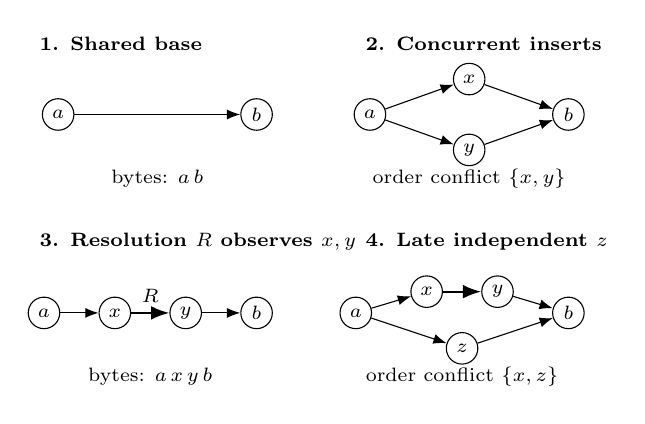
\begin{tikzpicture}[x=9mm,y=9mm,>=Latex,font=\scriptsize,
 atom/.style={circle,draw,inner sep=1.2pt,minimum size=4mm},
 title/.style={anchor=west,font=\scriptsize\bfseries}]
\node[title] at (0,2.5) {1. Shared base};
\node[atom] (a1) at (0.4,1.5) {$a$};
\node[atom] (b1) at (3.2,1.5) {$b$};
\draw[->] (a1)--(b1);
\node at (1.8,0.6) {bytes: $a\,b$};
\node[title] at (4.6,2.5) {2. Concurrent inserts};
\node[atom] (a2) at (4.8,1.5) {$a$};
\node[atom] (x2) at (6.2,2.0) {$x$};
\node[atom] (y2) at (6.2,1.0) {$y$};
\node[atom] (b2) at (7.6,1.5) {$b$};
\draw[->] (a2)--(x2);\draw[->] (x2)--(b2);
\draw[->] (a2)--(y2);\draw[->] (y2)--(b2);
\node at (6.2,0.6) {order conflict $\{x,y\}$};
\node[title] at (0,-0.3) {3. Resolution $R$ observes $x,y$};
\node[atom] (a3) at (0.2,-1.3) {$a$};
\node[atom] (x3) at (1.2,-1.3) {$x$};
\node[atom] (y3) at (2.2,-1.3) {$y$};
\node[atom] (b3) at (3.2,-1.3) {$b$};
\draw[->] (a3)--(x3);\draw[->,thick] (x3)--node[above] {$R$}(y3);\draw[->] (y3)--(b3);
\node at (1.7,-2.2) {bytes: $a\,x\,y\,b$};
\node[title] at (4.6,-0.3) {4. Late independent $z$};
\node[atom] (a4) at (4.6,-1.3) {$a$};
\node[atom] (x4) at (5.6,-1.0) {$x$};
\node[atom] (y4) at (6.6,-1.0) {$y$};
\node[atom] (z4) at (6.1,-1.8) {$z$};
\node[atom] (b4) at (7.6,-1.3) {$b$};
\draw[->] (a4)--(x4);\draw[->,thick] (x4)--(y4);\draw[->] (y4)--(b4);
\draw[->] (a4)--(z4);\draw[->] (z4)--(b4);
\node at (6.1,-2.2) {order conflict $\{x,z\}$};
\end{tikzpicture}
\caption{A resolution orders only what it observed. $R$ adds the edge $x\to y$. An independent $z$ inserted against the original base is unordered relative to $x$, so the view again has a conflict and no bytes. Transitive edges are omitted.}
\Description{Four document states: base atoms a then b; concurrent x and y inserted between them; a resolution adding x before y; and late independent z inserted between a and b, creating new ambiguity.}
\label{fig:conflicts}
\end{figure}

\subsection{Interval documents}\label{sec:interval}
The legacy representation edits a file as lines against one immutable base. An edit is a set of intervals $(s,e,c)$, each replacing base lines $[s,e)$ with the lines $c$. Two nonempty intervals \emph{conflict} when their ranges overlap. A zero-width interval (an insertion at $s=e$) conflicts with any interval whose closed range contains $s$, so an insertion exactly at the boundary of a replacement is a conflict rather than silently reordered across it. Two intervals with the same range and content are the same edit. A set of in-bounds, pairwise nonconflicting intervals, sorted by start, renders a unique byte string, so concurrent interval edits of one base merge in any order. This model does not reduce graph documents to intervals. It is the representation that the measured workloads use (Section~\ref{sec:evidence}) and the one that ordinary Git edits of legacy paths are imported into. Both representations have their own proofs.

\section{Verification with h5i-app}\label{sec:verification}
\subsection{Instantiating the kernel contract}\label{sec:toolchain}
\sys\ has two extracted kernels. The \emph{registry} kernel is the h5i-app transition of Equation~\ref{eq:kernel}. The \emph{document} kernel, \code{o5s\_kernel}, holds validation, commit, and materialization for graph documents, line merging for interval documents, and the head computation, and is called by the registry kernel and by the shell. Both are written in the Rust subset Charon and Aeneas translate, and both are extracted by h5i-app.

The registry kernel instantiates Equation~\ref{eq:kernel} as follows.
\begin{itemize}
\item The principal is $a=(\mathit{org},\mathit{user},\mathit{scope})$: the organization and user from the verified token, and the tenant the shell loaded, which is either one repository or one organization's directory of repository names.
\item The snapshot $s$ is one tenant's rows: the repository row with its counters, and the tables \code{patches}, \code{dependencies}, \code{approvals}, \code{checks}, \code{channels}, \code{members}, \code{paths}, \code{events}, \code{bodies}, \code{listings}, and \code{roles}. These are the state $S$ of Definition~\ref{def:state} stored relationally: a \code{patches} row is $(\mathit{id},h_p,\operatorname{author})$, \code{dependencies} is $D$, \code{approvals} is $A$, \code{checks} is $K$ (keyed by patch, so one row per patch), and a \code{members} row $(c,\mathit{position},p)$ is one element of $M_c$.
\item The command $c$ is one of the commands of Section~\ref{sec:commands} or a read-only load.
\item A write is a keyed upsert of one row (\code{PutPatch}, \code{PutApproval}, \code{PutMember}, \dots) or a replacement of the repository row, and $\operatorname{commit}(s,W)$ applies them in order.
\end{itemize}
Alongside the extracted kernel there is a hand-written Lean function $M(a,s,c)$, the \emph{model}, which is Definitions~\ref{def:state}--\ref{def:admission} written out over the same row types: role checks, hash deduplication, the independence refusals of $\mathbf{Approve}$ and $\mathbf{Check}$, and the fold of Equation~\ref{eq:gate} for $\mathbf{Merge}$. The model is 293 lines of Lean. The document kernel is related in the same way to the model of Sections~\ref{sec:documents} and~\ref{sec:views}.

\subsection{Registry theorems}\label{sec:registry}
Let $T(a,s,c)$ be the extracted registry transition. The \emph{registry invariant} $\operatorname{Inv}(s)$ is the conjunction of: patch handles and identities are unique and below the repository counters; every dependency names a registered, earlier patch; every approval and check report names a registered patch whose author differs from the reviewer or reporter; every channel's membership is dependency-closed (Equation~\ref{eq:closure}) and every member was approved; and an uncreated repository has no rows.

\begin{claim}[Refinement and invariant preservation]\label{thm:refine}
For every $a$, $s$, $c$: whenever $T(a,s,c)$ returns an outcome, a success $\Ok(W,\mathit{reply})$ or a refusal $\Err(e)$, that outcome equals $M(a,s,c)$. If $T(a,s,c)$ succeeds and $\operatorname{Inv}(s)$, then $\operatorname{Inv}(\operatorname{commit}(s,W))$. Consequently $\operatorname{Inv}$ holds in every state reachable from an empty tenant by successful commands; no successful command changes or removes a registered patch; and no successful command removes or reorders a channel member.
\end{claim}
\noindent\emph{Proof sketch.} The extracted helpers (finding a patch by hash, computing the dependency list, the admission fold) are first shown equal to their model counterparts, then \code{transition} is unfolded by cases on the command. Preservation is one lemma per command. For $\mathbf{Propose}$, the fresh handle is the incremented counter, so it cannot collide with an existing row. For $\mathbf{Merge}$, induction over the fold shows that each admitted patch's dependencies lie in the members so far, which gives Equation~\ref{eq:closure} for the result. Reachability is induction over command sequences. The Lean names are \code{Refine.transition\_refines}, \code{Invariant.inv\_preserved}, \code{reachable\_inv}, \code{patches\_immutable}, and \code{members\_append\_only}.

\begin{claim}[Admission gate and isolation]\label{thm:gate}
Suppose a $\mathbf{Merge}$ into channel $c$ succeeds in snapshot $s$ with write set $W$. Then for every member write $(c,\_,p)\in W$ the snapshot $s$ contains an approval of $p$ and a check report on $p$ with result $\mathit{pass}$. In every reachable state those approvals and reports come from identities other than $\operatorname{author}(p)$. A repository command succeeds only on a created repository whose organization is $a.\mathit{org}$, and a directory scope never writes repository rows or vice versa.
\end{claim}
\noindent\emph{Proof sketch.} By Theorem~\ref{thm:refine} the writes are the model's. The model's fold emits a member write for $p$ only after the two guards of Equation~\ref{eq:gate} succeed, and those guards read $A$ and $K$ from $s$ (\code{Guarantees.merge\_gate}). Independence is not part of the merge but of the invariant: the fields \code{approvals\_independent} and \code{checks\_independent} are established by $\mathbf{Approve}$ and $\mathbf{Check}$ and carried by \code{reachable\_inv}. The scope statements are \code{isolation} and \code{scopes\_separate}.

The gate reads the report present \emph{at admission}: because $K$ keeps one report per patch, a later report can replace it, and Theorem~\ref{thm:gate} does not say that admitted patches have a currently passing report. The report is also about one patch, not about the channel it joins: passing checks on $p$ and on $q$ do not establish anything about the program that contains both. A snapshot-level gate that binds a check to the exact combined channel view is future work.

\subsection{Document theorems}\label{sec:convergence}
The executable document, \code{document::Doc}, stores the history of Definition~\ref{def:history} with dense indices assigned in arrival order: anchors $0$ and $1$ are the sentinels, atoms follow in creation order, and tables hold edges with the operation that wrote them, deletion tags, restorations, acknowledgements, and retractions. The relation $\operatorname{Rep}(d,H)$ says that every table of the dense state $d$ is the image of the identity-level history $H$ under the interning map, and $\operatorname{Replayed}(d,H)$ says that $d$ was produced by validating and committing the patches of $H$ through the extracted functions. \emph{Room} conditions bound counts, indices, and output sizes by the machine's integer limits.

\begin{claim}[Order-independent materialization]\label{thm:converge}
Let $\operatorname{Replayed}(d_1,H_1)$ and $\operatorname{Replayed}(d_2,H_2)$ where $H_1$ and $H_2$ contain the same patches, possibly delivered in different orders, with distinct identities, and both states have room. Then the extracted materializer returns, for $d_1$ and $d_2$, results that decode to the same view of Definition~\ref{def:view}: the same layers, the same conflicts, and the same bytes when defined.
\end{claim}
\noindent\emph{Proof sketch.} (1) Simulation: for each of the six operations, the extracted validator refuses exactly when the model does, with the same error, and a validated commit preserves $\operatorname{Rep}$ (\code{DocRefine}). (2) Materialization refinement: the extracted liveness table equals $\Live_H$, the extracted boundary rows are exactly $\operatorname{Sum}_H$, and the Kahn loop's layers and blocked remainder match the depths and blocked set of Section~\ref{sec:views}. Composed, these show that the decoded result satisfies the view specification (\code{DocMatRefine.materialize\_refines}). (3) Model: the view specification depends only on the \emph{set} of patches, and any two views of one history are equal (\code{view\_perm}, \code{view\_unique}). Distinct identities and equal patch sets make $H_1$ a permutation of $H_2$, which closes the argument (\code{extracted\_view\_converges}).

The model also proves that validation of a patch reads only $\Obs(p)$, that two concurrent admissions commute, and that a patch refused for anything but missing dependencies is refused in every delivery order (\code{DocModel.validate\_local}, \code{apply\_comm}, \code{admissible\_any\_order}). Theorem~\ref{thm:converge} is therefore about every \emph{complete} delivery that respects dependencies, and it does not say that deliveries complete. For interval documents the corresponding results are \code{Lines.merge\_order\_independent} and \code{merged\_renders}: two sorted arrangements of the same nonconflicting intervals merge identically and always render.

\subsection{Causal heads}\label{sec:heads}
A workspace proposal must name, as $\deps(p)$, what its author saw, which is the exported channel view. Naming every member would make dependency lists grow with history. Let $\heads(C)$ be the members of a dependency-closed $C$ on which no other member directly depends.
\begin{claim}[Heads cover the past]\label{thm:heads}
For a dependency-closed channel $C$ whose dependency rows form a DAG, the extracted head computation returns a sublist of $C$, none of whose elements is a dependency of a member, and
\begin{equation}
 \past(\heads(C))=\past(C)=C.
 \label{eq:heads}
\end{equation}
\end{claim}
\noindent\emph{Proof sketch.} Every member either is a head or is a dependency of some member. Following dependency edges upward from any member reaches a head because the graph is finite and acyclic, so every member is in the past of some head. Heads are members, so the converse inclusion holds (\code{Heads.heads\_keep\_past}). The native workspace adapter is responsible for binding the heads it names to the snapshot it actually exported.

\subsection{Trusted computing base}\label{sec:gate}
The proofs are complete and axiom-free: no theorem depends on \code{sorry}, \code{native\_decide}, or any axiom beyond Lean's \code{propext}, \code{Classical.choice}, and \code{Quot.sound}. The Lean they are about is regenerated from the current Rust source and compared byte for byte with the translation the proofs were checked against, so a change to a kernel that is not reflected in the proofs is detected. The full statements, with all hypotheses, are in the repository~\cite{o5s}.

\section{System architecture}\label{sec:architecture}
\begin{figure}[t]
\centering
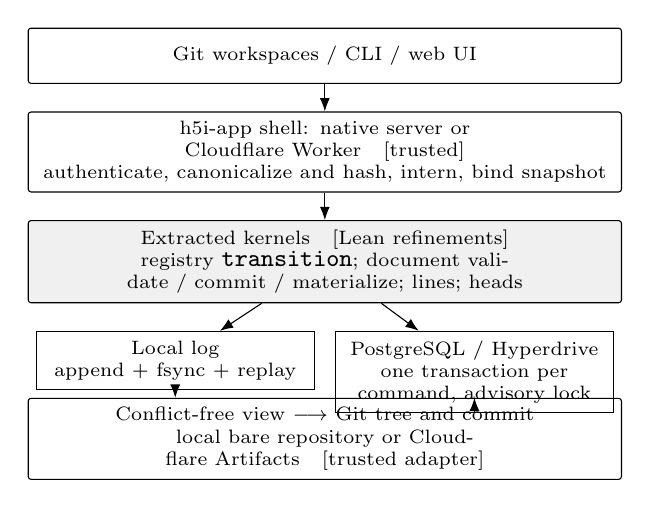
\begin{tikzpicture}[font=\scriptsize,>=Latex,node distance=3.5mm,
 box/.style={draw,rounded corners=1pt,align=center,minimum height=7mm,text width=73mm},
 half/.style={draw,align=center,minimum height=7mm,text width=33mm}]
\node[box] (agents) {Git workspaces / CLI / web UI};
\node[box,below=of agents] (adapter) {h5i-app shell: native server or Cloudflare Worker\quad [trusted]\par authenticate, canonicalize and hash, intern, bind snapshot};
\node[box,below=of adapter,fill=black!6] (kernel) {Extracted kernels\quad [Lean refinements]\par registry \code{transition}; document validate / commit / materialize; lines; heads};
\node[half,below=of kernel,xshift=-19mm] (wal) {Local log\par append + fsync + replay};
\node[half,below=of kernel,xshift=19mm] (pg) {PostgreSQL / Hyperdrive\par one transaction per command, advisory lock};
\node[box,below=12mm of kernel] (projection) {Conflict-free view $\longrightarrow$ Git tree and commit\par local bare repository or Cloudflare Artifacts\quad [trusted adapter]};
\draw[->] (agents)--(adapter);
\draw[->] (adapter)--(kernel);
\draw[->] (kernel)--(wal);
\draw[->] (kernel)--(pg);
\draw[->] (wal.south)--(projection.north -| wal.south);
\draw[->] (pg.south)--(projection.north -| pg.south);
\end{tikzpicture}
\caption{One decision kernel, two durable backends, and derived Git projections. The shaded layer is the extracted code, and everything else is the shell with explicit obligations.}
\Description{Agents reach an h5i-app shell, which calls the extracted registry and document kernels. Writes commit to a local log or to PostgreSQL. Conflict-free views become Git projections through trusted adapters.}
\label{fig:architecture}
\end{figure}

\subsection{Prepare, decide, commit}\label{sec:commit}
A request passes through three stages (Fig.~\ref{fig:architecture}). \emph{Prepare}: the shell authenticates the caller, canonicalizes and hashes the proposed patch body, interns the identities it names into handles, and loads the tenant's rows. \emph{Decide}: the registry kernel returns a refusal or a write set, calling the document kernel to validate graph operations and \code{patch::merge} to admit members. \emph{Commit}: a storage engine applies the write set atomically. The native server and the Cloudflare Worker call the same \code{transition}, so the engines differ only in persistence, not in policy.

The local engine appends each decided command, with its SHA-256 checksum, to a write-ahead log, calls \code{fdatasync} before acknowledging, and replays the log through the kernel's \code{commit} at startup. The PostgreSQL engine runs each command as one \code{READ COMMITTED} transaction that first takes a transaction-scoped advisory lock on the tenant (a repository, or an organization's directory). The lock orders all commands of a tenant, and commands of different tenants touch disjoint rows. This replaced an earlier engine that used \code{SERIALIZABLE} isolation (h5i-app's default), whose predicate locks on shared index pages made unrelated repositories abort each other. Under the lock, a run that previously retried 3,570 of 15,598 attempts retried none.

Two storage optimizations have model-level proofs. A command loads only the rows it can read (\code{Narrow.narrow\_load}: a transition on a partial snapshot equals the transition on the full one when the loaded rows agree on every lookup the command performs), and the PostgreSQL loader is modeled branch by branch and shown to return such rows for reachable states whose dependency lists are stored in key order (\code{Served.pg\_served}). The native server also groups commands that arrive while a tenant's transaction is open into the next transaction, keeping the repository counter row in memory and writing it once. \code{Group.group\_served} and \code{defer\_repo} show that each grouped command sees the state the earlier ones left. Idempotency keys bind a command fingerprint and its reply to the committing transaction, so a retry after an unknown commit outcome returns the stored reply instead of deciding twice.

\subsection{Git as projection and workspace}\label{sec:gitinterface}
Git is the interface, not the store of record. Agents edit ordinary Git worktrees checked out from an \emph{exported snapshot}: a channel view whose $\operatorname{bytes}$ are defined for every path, written as Git trees and a commit whose message records the channel's generation and causal heads. A proposal is the difference between the worktree and that snapshot, with $\deps(p)=\heads(C)$ by Theorem~\ref{thm:heads}, translated into graph operations against the atoms of the exported view, or into intervals for legacy paths. A view with an open conflict is not exported, so unresolved alternatives never appear as a Git tree. They are resolved by a patch like any other.

The Cloudflare deployment reaches PostgreSQL through Hyperdrive and keeps projections and per-agent workspace repositories in Artifacts. The Worker builds Git objects and pushes a pack, and workspace imports read trees and blobs from the Artifacts binding. A merge records its pending export inside the same database transaction, a scheduled task retries undelivered exports, and generation checks with compare-and-swap reference updates stop an older export from overwriting a newer one. These adapters are tested, not proved.

\section{Related systems}\label{sec:related}
\emph{Git.} A commit's identity includes its parents~\cite{gitobjects}, so integrating a change onto a moved branch rewrites it~\cite{gitrebase}, and whether review carries over is a hosting policy. \sys\ admits an unchanged identity into a set. Hosted Git can enforce review and checks through branch protection and hooks. The difference is not the policy but that \sys's policy is an extracted function with a refinement proof and an invariant that holds in every reachable state.

\emph{Darcs and Pijul.} Darcs reasons about commutation of context-sensitive patches~\cite{darcs}. Pijul represents text as a graph with explicit dependencies and keeps conflicts in the repository~\cite{pijul}. \sys\ takes stable atom identity, observed context, channels, and conflict retention from this line of work. Its document model is deliberately smaller: six operations, deletion as tags, and order edges with retraction, rather than Pijul's edge-label algebra or Darcs's general patch inversion. The claim is not equivalence to either system but that this bounded model is implemented by proved code.

\emph{Theories of patches.} Mimram and Di Giusto model merging categorically and show why a merge representation must contain unresolved states~\cite{patches}. Angiuli et al.\ represent patch theories as higher inductive types~\cite{homotopical}. These works give the design principle that conflicts are objects. \sys's contribution is on the implementation side of that principle: the Rust validator, commit, and materializer are shown to realize the identity-level model of Section~\ref{sec:model}.

\emph{CRDTs and Jujutsu.} Sequence CRDTs converge by making concurrent operations commute, and Gomes et al.\ verified that property in Isabelle/HOL together with a network model~\cite{sec}. \sys\ shares the causal-delivery setting but converges on a \emph{conflict-bearing} view rather than on text, and leaves delivery to the shell. Jujutsu also stores conflicted states in commits and allows further work before resolution~\cite{jj} but does not aim at a verified admission policy.

\section{Preliminary evaluation}\label{sec:evidence}
Table~\ref{tab:measurements} compares \sys\ with unattended Git. The host was a 128-thread AMD EPYC 7502 with 251\,GiB of memory, running clients and server together. The \sys\ server used the local-log engine in a release build. Git 2.43.0 used pre-created clones and a \code{file://} remote, so the Git side paid for no server, authentication, or network. Each run had 1,000 agents with at most 64 requests in flight. A Git agent pushed, and on rejection pulled with rebase and pushed again, and a rebase conflict stopped it. An \sys\ agent proposed, an independent identity approved and reported a passing check, and patches were merged in batches of 100. The shared-file workloads used interval proposals (Section~\ref{sec:interval}), not graph documents, and the check reports were generated by the load driver, not by running a test suite. Final contents were checked in every run.

\begin{table}[t]
\caption{Recorded integrations per second, 1,000 agents on one host. Every \sys\ run admitted all 1,000 proposals. \emph{API} agents call the HTTP API directly, and \emph{CLI} agents run \code{o5s propose} in their own Git repository.}
\label{tab:measurements}
\centering\small
\begin{tabular}{@{}lrrrr@{}}
\toprule
Workload & Git integrated & Git/s & \sys\ API/s & \sys\ CLI/s\\
\midrule
Adjacent lines, one file & 431 & 9.8 & 574 & 145\\
Lines four apart, one file & 1,000 & 5.0 & 244 & 48\\
One new file each & 1,000 & 9.0 & 1,083 & 245\\
Same line, one file & 1 & --- & $595^{*}$ & $146^{*}$\\
\bottomrule
\end{tabular}
\par\vspace{2pt}\footnotesize $^{*}$Admitted as retained conflict alternatives, so a resolution patch is still needed.
\end{table}

Where agents edit one shared file, Git's throughput is bounded by the rebase loop regardless of whether the edits conflict (the four-apart row has no conflicts and 55,773 push retries), and adjacent edits stop 569 of 1,000 agents, whereas \sys\ admits all of them because disjoint intervals of one base merge as a set. The CLI rows include process start-up and worktree reads for each proposal, whereas the API rows measure the server alone. On the same line, neither system chooses a winner: Git stops 999 agents, each with a local conflict, and \sys\ keeps all 1,000 alternatives in one place for one reviewed resolution.

The Git baseline is one unattended workflow without a merge queue, custom merge drivers, or human conflict resolution, and the measurements are closed-loop on one host. Multi-host and adversarial evaluations, and load on the graph document path, remain open.

\section{Conclusion}
We presented \sys, a patch-based collaboration server for agent swarms whose Rust decision kernel is formally verified in Lean~4 against a model of review-gated, conflict-preserving version control. The proofs establish that the kernel refines the model and preserves dependency closure and independent review in every reachable state, that a patch is admitted only with an approval and a passing check from identities other than its author, that materialization of a graph document is independent of delivery order, and that the causal heads a workspace names cover the snapshot it saw. The same kernel serves a local log, PostgreSQL, and Cloudflare Workers with Artifacts, and agents interact with it through ordinary Git checkouts. With 1,000 agents on one repository, \sys\ admits every proposal at 244 to 1,083 integrations per second across the measured workloads, whereas on adjacent lines of one file unattended Git integrates 9.8 changes per second and stops 569 of the agents at rebase conflicts.

\bibliographystyle{ACM-Reference-Format}
\bibliography{o5s-references}
\end{document}
